\documentclass[11pt,]{article}
\usepackage[]{mathpazo}
\usepackage{amssymb,amsmath}
\usepackage{ifxetex,ifluatex}
\usepackage{fixltx2e} % provides \textsubscript
\ifnum 0\ifxetex 1\fi\ifluatex 1\fi=0 % if pdftex
  \usepackage[T1]{fontenc}
  \usepackage[utf8]{inputenc}
\else % if luatex or xelatex
  \ifxetex
    \usepackage{mathspec}
  \else
    \usepackage{fontspec}
  \fi
  \defaultfontfeatures{Ligatures=TeX,Scale=MatchLowercase}
\fi
% use upquote if available, for straight quotes in verbatim environments
\IfFileExists{upquote.sty}{\usepackage{upquote}}{}
% use microtype if available
\IfFileExists{microtype.sty}{%
\usepackage{microtype}
\UseMicrotypeSet[protrusion]{basicmath} % disable protrusion for tt fonts
}{}
\usepackage[margin = 1in]{geometry}
\usepackage{hyperref}
\hypersetup{unicode=true,
            pdfauthor={Brandon Hufstetler, Garrett Alarcon, Jinan Andrews, Anson Cheng, Nick Forrest, and Nestor Herandez},
            pdfborder={0 0 0},
            breaklinks=true}
\urlstyle{same}  % don't use monospace font for urls
\usepackage{color}
\usepackage{fancyvrb}
\newcommand{\VerbBar}{|}
\newcommand{\VERB}{\Verb[commandchars=\\\{\}]}
\DefineVerbatimEnvironment{Highlighting}{Verbatim}{commandchars=\\\{\}}
% Add ',fontsize=\small' for more characters per line
\usepackage{framed}
\definecolor{shadecolor}{RGB}{248,248,248}
\newenvironment{Shaded}{\begin{snugshade}}{\end{snugshade}}
\newcommand{\AlertTok}[1]{\textcolor[rgb]{0.94,0.16,0.16}{#1}}
\newcommand{\AnnotationTok}[1]{\textcolor[rgb]{0.56,0.35,0.01}{\textbf{\textit{#1}}}}
\newcommand{\AttributeTok}[1]{\textcolor[rgb]{0.77,0.63,0.00}{#1}}
\newcommand{\BaseNTok}[1]{\textcolor[rgb]{0.00,0.00,0.81}{#1}}
\newcommand{\BuiltInTok}[1]{#1}
\newcommand{\CharTok}[1]{\textcolor[rgb]{0.31,0.60,0.02}{#1}}
\newcommand{\CommentTok}[1]{\textcolor[rgb]{0.56,0.35,0.01}{\textit{#1}}}
\newcommand{\CommentVarTok}[1]{\textcolor[rgb]{0.56,0.35,0.01}{\textbf{\textit{#1}}}}
\newcommand{\ConstantTok}[1]{\textcolor[rgb]{0.00,0.00,0.00}{#1}}
\newcommand{\ControlFlowTok}[1]{\textcolor[rgb]{0.13,0.29,0.53}{\textbf{#1}}}
\newcommand{\DataTypeTok}[1]{\textcolor[rgb]{0.13,0.29,0.53}{#1}}
\newcommand{\DecValTok}[1]{\textcolor[rgb]{0.00,0.00,0.81}{#1}}
\newcommand{\DocumentationTok}[1]{\textcolor[rgb]{0.56,0.35,0.01}{\textbf{\textit{#1}}}}
\newcommand{\ErrorTok}[1]{\textcolor[rgb]{0.64,0.00,0.00}{\textbf{#1}}}
\newcommand{\ExtensionTok}[1]{#1}
\newcommand{\FloatTok}[1]{\textcolor[rgb]{0.00,0.00,0.81}{#1}}
\newcommand{\FunctionTok}[1]{\textcolor[rgb]{0.00,0.00,0.00}{#1}}
\newcommand{\ImportTok}[1]{#1}
\newcommand{\InformationTok}[1]{\textcolor[rgb]{0.56,0.35,0.01}{\textbf{\textit{#1}}}}
\newcommand{\KeywordTok}[1]{\textcolor[rgb]{0.13,0.29,0.53}{\textbf{#1}}}
\newcommand{\NormalTok}[1]{#1}
\newcommand{\OperatorTok}[1]{\textcolor[rgb]{0.81,0.36,0.00}{\textbf{#1}}}
\newcommand{\OtherTok}[1]{\textcolor[rgb]{0.56,0.35,0.01}{#1}}
\newcommand{\PreprocessorTok}[1]{\textcolor[rgb]{0.56,0.35,0.01}{\textit{#1}}}
\newcommand{\RegionMarkerTok}[1]{#1}
\newcommand{\SpecialCharTok}[1]{\textcolor[rgb]{0.00,0.00,0.00}{#1}}
\newcommand{\SpecialStringTok}[1]{\textcolor[rgb]{0.31,0.60,0.02}{#1}}
\newcommand{\StringTok}[1]{\textcolor[rgb]{0.31,0.60,0.02}{#1}}
\newcommand{\VariableTok}[1]{\textcolor[rgb]{0.00,0.00,0.00}{#1}}
\newcommand{\VerbatimStringTok}[1]{\textcolor[rgb]{0.31,0.60,0.02}{#1}}
\newcommand{\WarningTok}[1]{\textcolor[rgb]{0.56,0.35,0.01}{\textbf{\textit{#1}}}}
\usepackage{graphicx,grffile}
\makeatletter
\def\maxwidth{\ifdim\Gin@nat@width>\linewidth\linewidth\else\Gin@nat@width\fi}
\def\maxheight{\ifdim\Gin@nat@height>\textheight\textheight\else\Gin@nat@height\fi}
\makeatother
% Scale images if necessary, so that they will not overflow the page
% margins by default, and it is still possible to overwrite the defaults
% using explicit options in \includegraphics[width, height, ...]{}
\setkeys{Gin}{width=\maxwidth,height=\maxheight,keepaspectratio}
\IfFileExists{parskip.sty}{%
\usepackage{parskip}
}{% else
\setlength{\parindent}{0pt}
\setlength{\parskip}{6pt plus 2pt minus 1pt}
}
\setlength{\emergencystretch}{3em}  % prevent overfull lines
\providecommand{\tightlist}{%
  \setlength{\itemsep}{0pt}\setlength{\parskip}{0pt}}
\setcounter{secnumdepth}{0}
% Redefines (sub)paragraphs to behave more like sections
\ifx\paragraph\undefined\else
\let\oldparagraph\paragraph
\renewcommand{\paragraph}[1]{\oldparagraph{#1}\mbox{}}
\fi
\ifx\subparagraph\undefined\else
\let\oldsubparagraph\subparagraph
\renewcommand{\subparagraph}[1]{\oldsubparagraph{#1}\mbox{}}
\fi

%%% Use protect on footnotes to avoid problems with footnotes in titles
\let\rmarkdownfootnote\footnote%
\def\footnote{\protect\rmarkdownfootnote}

%%% Change title format to be more compact
\usepackage{titling}

% Create subtitle command for use in maketitle
\providecommand{\subtitle}[1]{
  \posttitle{
    \begin{center}\large#1\end{center}
    }
}

\setlength{\droptitle}{-2em}

  \title{IMGT680 Homework 1}
    \pretitle{\vspace{\droptitle}\centering\huge}
  \posttitle{\par}
    \author{Brandon Hufstetler, Garrett Alarcon, Jinan Andrews, Anson Cheng, Nick
Forrest, and Nestor Herandez}
    \preauthor{\centering\large\emph}
  \postauthor{\par}
      \predate{\centering\large\emph}
  \postdate{\par}
    \date{1 July 2019}

\usepackage{fancyhdr}
\pagestyle{fancy}
\fancyfoot[CO,CE]{Forrest - Page \thepage}

\begin{document}
\maketitle

\hypertarget{chapter-1}{%
\section{Chapter 1}\label{chapter-1}}

\hypertarget{getting-started-with-r}{%
\subsection{GETTING STARTED WITH R}\label{getting-started-with-r}}

\hypertarget{comments-indents-and-semicolons}{%
\subsubsection{Comments, indents, and
semicolons}\label{comments-indents-and-semicolons}}

\begin{Shaded}
\begin{Highlighting}[]
  \CommentTok{# Anything prefaced by a pound sign (#) is a comment.}
  \CommentTok{# Comments are not executed by R. Instead, they explain what the code is doing.}
  \CommentTok{# Indented code (that is not a comment) will run in R as if it was on one line}
  \CommentTok{# Code separated by semicolons will run as if the code was on separate lines,}
  \CommentTok{# with the semicolon marking the line break}
\end{Highlighting}
\end{Shaded}

\hypertarget{open-a-dataset-and-display-the-data}{%
\subsubsection{Open a dataset and display the
data}\label{open-a-dataset-and-display-the-data}}

\hypertarget{the-setwd-command-is-used-to-make-imgt680-the-working-directory.}{%
\paragraph{The setwd() command is used to make \textasciitilde{}/IMGT680
the working
directory.}\label{the-setwd-command-is-used-to-make-imgt680-the-working-directory.}}

\begin{Shaded}
\begin{Highlighting}[]
\NormalTok{  filepath <-}\StringTok{ ""}
  \KeywordTok{setwd}\NormalTok{(}\StringTok{"~/IMGT680"}\NormalTok{)}
\NormalTok{  cars <-}\StringTok{ }\KeywordTok{read.csv}\NormalTok{(}\DataTypeTok{file =} \StringTok{"cars.txt"}\NormalTok{, }\DataTypeTok{stringsAsFactors =} \OtherTok{FALSE}\NormalTok{)}
\NormalTok{  cars }\CommentTok{# To display the whole dataset, type the dataset name}
\end{Highlighting}
\end{Shaded}

\begin{Shaded}
\begin{Highlighting}[]
  \KeywordTok{head}\NormalTok{(cars) }\CommentTok{# Display the first few records of a dataset}
\end{Highlighting}
\end{Shaded}

\begin{verbatim}
##    mpg cylinders cubicinches  hp weightlbs time.to.60 year    brand
## 1 14.0         8         350 165      4209         12 1972      US.
## 2 31.9         4          89  71      1925         14 1980  Europe.
## 3 17.0         8         302 140      3449         11 1971      US.
## 4 15.0         8         400 150      3761         10 1971      US.
## 5 30.5         4          98  63      2051         17 1978      US.
## 6 23.0         8         350 125      3900         17 1980      US.
\end{verbatim}

\begin{Shaded}
\begin{Highlighting}[]
  \KeywordTok{names}\NormalTok{(cars) }\CommentTok{# Display variable names of a data frame, one kind of data in R}
\end{Highlighting}
\end{Shaded}

\begin{verbatim}
## [1] "mpg"         "cylinders"   "cubicinches" "hp"          "weightlbs"  
## [6] "time.to.60"  "year"        "brand"
\end{verbatim}

\begin{Shaded}
\begin{Highlighting}[]
\NormalTok{  cars}\OperatorTok{$}\NormalTok{weight }\CommentTok{# Look at only the weight variable within data frame cars}
\end{Highlighting}
\end{Shaded}

\begin{verbatim}
##   [1] 4209 1925 3449 3761 2051 3900 4363 4312 3530 2050 2245 2188 4141 3664
##  [15] 3381 4360 2020 3433 2278 2430 2019 2600 3012 4054 1968 1795 1773 4657
##  [29] 3574 2380 2130 3278 2506 2648 1985 3415 1835 2720 3955 3265 3897 4638
##  [43] 3645 3520 3086 2635 3755 2395 1940 3060 4464 3190 3609 2158 4380 4278
##  [57] 2930 2075 1937 3821 2945 2379 2910 2110 4237 3525 1950 1965 1825 3880
##  [71] 3102 2640 2288 2545 2219 3015 3085 2515 2265 2350 4325 4952 3425 2694
##  [85] 2220 1613 2774 3465 2125 2720 1975 2300 4100 3329 2255 3907 4499 3139
##  [99] 3830 3781 4997 4906 2126 2200 2265 2635 2335 2065 2671 3504 2279 2933
## [113] 4335 1795 2130 3785 2740 3039 2045 4341 2202 1963 4668 2745 1834 2565
## [127] 4654 2230 2582 1800 2300 2678 4951 3672 4440 4190 1955 3169 2945 2979
## [141] 2700 2171 2665 1760 3605 2957 3360 2735 3693 3205 2542 2560 4425 3158
## [155] 2464 3302 2124 2135 2634 3410 3003 4080 2984 2904 2254 3365 3439 2585
## [169] 2807 2125 2290 2830 1867 2575 2226 2189 4385 3672 3570 2045 2990 2145
## [183] 4215 3436 2395 3070 3459 3940 4129 4735 2620 2670 4422 4082 4077 2144
## [197] 2490 1985 1937 1945 2246 2639 3420 3630 2401 3850 2110 3021 4098 2900
## [211] 2815 3445 1755 2074 3233 2615 1975 4215 2595 4295 3193 2795 4457 3820
## [225] 4042 2003 4615 1649 2587 2790 3563 2625 2592 4498 3150 2130 4096 2965
## [239] 1875 2220 4055 3121 4220 2672 4354 3399 3735 2085 2155 2525 2120 2660
## [253] 2950 3988 2725 2372 3840 1800 2835 3288 3353
\end{verbatim}

\hypertarget{matrices}{%
\subsection{Matrices}\label{matrices}}

\hypertarget{create-a-matrix-with-three-rows-two-columns-and-every-value-equal-to-0.0}{%
\subsubsection{Create a matrix with three rows, two columns, and every
value equal to
0.0}\label{create-a-matrix-with-three-rows-two-columns-and-every-value-equal-to-0.0}}

\begin{Shaded}
\begin{Highlighting}[]
\NormalTok{  mat <-}\StringTok{ }\KeywordTok{matrix}\NormalTok{(}\FloatTok{0.0}\NormalTok{, }\DataTypeTok{nrow =} \DecValTok{3}\NormalTok{, }\DataTypeTok{ncol =} \DecValTok{2}\NormalTok{); mat}
\end{Highlighting}
\end{Shaded}

\begin{verbatim}
##      [,1] [,2]
## [1,]    0    0
## [2,]    0    0
## [3,]    0    0
\end{verbatim}

\begin{Shaded}
\begin{Highlighting}[]
  \KeywordTok{colnames}\NormalTok{(mat) <-}\StringTok{ }\KeywordTok{c}\NormalTok{(}\StringTok{"Var 1"}\NormalTok{, }\StringTok{"Var 2"}\NormalTok{) }\CommentTok{# Give a matrix variable names}
  \KeywordTok{colnames}\NormalTok{(mat) }\CommentTok{# Display variable names of a matrix}
\end{Highlighting}
\end{Shaded}

\begin{verbatim}
## [1] "Var 1" "Var 2"
\end{verbatim}

\hypertarget{subset-data-and-declare-new-variables}{%
\subsubsection{Subset data and declare new
variables}\label{subset-data-and-declare-new-variables}}

\begin{Shaded}
\begin{Highlighting}[]
\NormalTok{  cars.rsub <-}\StringTok{ }\NormalTok{cars[}\DecValTok{1}\OperatorTok{:}\DecValTok{50}\NormalTok{,] }\CommentTok{# Subset the data by rows}
\NormalTok{  cars.csub <-}\StringTok{ }\NormalTok{cars[,}\DecValTok{1}\OperatorTok{:}\DecValTok{3}\NormalTok{] }\CommentTok{# Subset by columns}
\NormalTok{  cars.rcsub <-}\StringTok{ }\NormalTok{cars[}\KeywordTok{c}\NormalTok{(}\DecValTok{1}\NormalTok{,}\DecValTok{3}\NormalTok{,}\DecValTok{5}\NormalTok{), }\KeywordTok{c}\NormalTok{(}\DecValTok{2}\NormalTok{,}\DecValTok{4}\NormalTok{)] }\CommentTok{# Subset by specific rows and columns}
\NormalTok{  cars.vsub <-}\StringTok{ }\NormalTok{cars[}\KeywordTok{which}\NormalTok{(cars}\OperatorTok{$}\NormalTok{mpg}\OperatorTok{>}\StringTok{ }\DecValTok{30}\NormalTok{),] }\CommentTok{# Subset by a logical condition}
\CommentTok{# To declare new variables, type the variable name, a left-arrow, then the value of the variable}
\NormalTok{  firstletter <-}\StringTok{ 'a'}
\NormalTok{  weight <-}\StringTok{ }\NormalTok{cars}\OperatorTok{$}\NormalTok{weight}
\end{Highlighting}
\end{Shaded}

\hypertarget{display-more-than-one-figure-at-a-time}{%
\subsubsection{Display more than one figure at a
time}\label{display-more-than-one-figure-at-a-time}}

\begin{Shaded}
\begin{Highlighting}[]
  \KeywordTok{par}\NormalTok{(}\DataTypeTok{mfrow=}\KeywordTok{c}\NormalTok{(}\DecValTok{1}\NormalTok{,}\DecValTok{1}\NormalTok{)) }\CommentTok{# plots one figure; the default setting}
  \KeywordTok{par}\NormalTok{(}\DataTypeTok{mfrow=}\KeywordTok{c}\NormalTok{(}\DecValTok{2}\NormalTok{,}\DecValTok{3}\NormalTok{)) }\CommentTok{# plots six figures: three in the top row, three in the bottom row}
  \CommentTok{# Plots will fill the plot space row by row}
\end{Highlighting}
\end{Shaded}

\hypertarget{download-and-install-an-r-package}{%
\subsubsection{Download and install an R
Package}\label{download-and-install-an-r-package}}

\begin{Shaded}
\begin{Highlighting}[]
  \CommentTok{#install.packages("ggplot2")}
  \KeywordTok{library}\NormalTok{(ggplot2)}
\end{Highlighting}
\end{Shaded}

\hypertarget{chapter-2}{%
\section{Chapter 2}\label{chapter-2}}

\hypertarget{read-in-the-cars-and-cars2-datasets}{%
\subsubsection{READ IN THE CARS AND CARS2
DATASETS}\label{read-in-the-cars-and-cars2-datasets}}

\begin{Shaded}
\begin{Highlighting}[]
  \KeywordTok{setwd}\NormalTok{(}\StringTok{"~/IMGT680"}\NormalTok{)}
\NormalTok{  cars <-}\StringTok{ }\KeywordTok{read.csv}\NormalTok{(}\StringTok{"cars.txt"}\NormalTok{, }\DataTypeTok{stringsAsFactors =} \OtherTok{FALSE}\NormalTok{)}
\NormalTok{  cars2 <-}\StringTok{ }\KeywordTok{read.csv}\NormalTok{(}\StringTok{"cars2.txt"}\NormalTok{, }\DataTypeTok{stringsAsFactors =} \OtherTok{FALSE}\NormalTok{)}
\end{Highlighting}
\end{Shaded}

\hypertarget{missing-data}{%
\subsubsection{MISSING DATA}\label{missing-data}}

\begin{Shaded}
\begin{Highlighting}[]
  \CommentTok{# Look at four variables from cars}
\NormalTok{  cars}\FloatTok{.4}\NormalTok{var <-}\StringTok{ }\NormalTok{cars[, }\KeywordTok{c}\NormalTok{(}\DecValTok{1}\NormalTok{, }\DecValTok{3}\NormalTok{, }\DecValTok{4}\NormalTok{, }\DecValTok{8}\NormalTok{)]}
  \KeywordTok{head}\NormalTok{(cars}\FloatTok{.4}\NormalTok{var)}
\end{Highlighting}
\end{Shaded}

\begin{verbatim}
##    mpg cubicinches  hp    brand
## 1 14.0         350 165      US.
## 2 31.9          89  71  Europe.
## 3 17.0         302 140      US.
## 4 15.0         400 150      US.
## 5 30.5          98  63      US.
## 6 23.0         350 125      US.
\end{verbatim}

\begin{Shaded}
\begin{Highlighting}[]
  \CommentTok{# Make certain entries missing}
\NormalTok{  cars}\FloatTok{.4}\NormalTok{var[}\DecValTok{2}\NormalTok{,}\DecValTok{2}\NormalTok{] <-}\StringTok{ }\NormalTok{cars}\FloatTok{.4}\NormalTok{var[}\DecValTok{4}\NormalTok{,}\DecValTok{4}\NormalTok{] <-}\StringTok{ }\OtherTok{NA}
  \KeywordTok{head}\NormalTok{(cars}\FloatTok{.4}\NormalTok{var)}
\end{Highlighting}
\end{Shaded}

\begin{verbatim}
##    mpg cubicinches  hp    brand
## 1 14.0         350 165      US.
## 2 31.9          NA  71  Europe.
## 3 17.0         302 140      US.
## 4 15.0         400 150     <NA>
## 5 30.5          98  63      US.
## 6 23.0         350 125      US.
\end{verbatim}

\begin{Shaded}
\begin{Highlighting}[]
  \CommentTok{# Replace missing values with constants}
\NormalTok{  cars}\FloatTok{.4}\NormalTok{var[}\DecValTok{2}\NormalTok{,}\DecValTok{2}\NormalTok{] <-}\StringTok{ }\DecValTok{0}
\NormalTok{  cars}\FloatTok{.4}\NormalTok{var[}\DecValTok{4}\NormalTok{,}\DecValTok{4}\NormalTok{] <-}\StringTok{ "Missing"}
  \KeywordTok{head}\NormalTok{(cars}\FloatTok{.4}\NormalTok{var)}
\end{Highlighting}
\end{Shaded}

\begin{verbatim}
##    mpg cubicinches  hp    brand
## 1 14.0         350 165      US.
## 2 31.9           0  71  Europe.
## 3 17.0         302 140      US.
## 4 15.0         400 150  Missing
## 5 30.5          98  63      US.
## 6 23.0         350 125      US.
\end{verbatim}

\begin{Shaded}
\begin{Highlighting}[]
  \CommentTok{# Replace values with mean and mode}
\NormalTok{  cars}\FloatTok{.4}\NormalTok{var[}\DecValTok{2}\NormalTok{,}\DecValTok{2}\NormalTok{] <-}\StringTok{ }\KeywordTok{mean}\NormalTok{(}\KeywordTok{na.omit}\NormalTok{(cars}\FloatTok{.4}\NormalTok{var}\OperatorTok{$}\NormalTok{cubicinches))}
\NormalTok{  our_table <-}\StringTok{ }\KeywordTok{table}\NormalTok{(cars}\FloatTok{.4}\NormalTok{var}\OperatorTok{$}\NormalTok{brand)}
\NormalTok{  our_mode <-}\StringTok{ }\KeywordTok{names}\NormalTok{(our_table)[our_table }\OperatorTok{==}\StringTok{ }\KeywordTok{max}\NormalTok{(our_table)]}
\NormalTok{  cars}\FloatTok{.4}\NormalTok{var[}\DecValTok{4}\NormalTok{,}\DecValTok{4}\NormalTok{] <-}\StringTok{ }\NormalTok{our_mode}
  \KeywordTok{head}\NormalTok{(cars}\FloatTok{.4}\NormalTok{var)}
\end{Highlighting}
\end{Shaded}

\begin{verbatim}
##    mpg cubicinches  hp    brand
## 1 14.0    350.0000 165      US.
## 2 31.9    200.7625  71  Europe.
## 3 17.0    302.0000 140      US.
## 4 15.0    400.0000 150      US.
## 5 30.5     98.0000  63      US.
## 6 23.0    350.0000 125      US.
\end{verbatim}

\begin{Shaded}
\begin{Highlighting}[]
  \CommentTok{# Generate random observations}
\NormalTok{  obs_brand <-}\StringTok{ }\KeywordTok{sample}\NormalTok{(}\KeywordTok{na.omit}\NormalTok{(cars}\FloatTok{.4}\NormalTok{var}\OperatorTok{$}\NormalTok{brand), }\DecValTok{1}\NormalTok{)}
\NormalTok{  obs_cubicinches <-}\StringTok{ }\KeywordTok{sample}\NormalTok{(}\KeywordTok{na.omit}\NormalTok{(cars}\FloatTok{.4}\NormalTok{var}\OperatorTok{$}\NormalTok{cubicinches), }\DecValTok{1}\NormalTok{)}
\NormalTok{  cars}\FloatTok{.4}\NormalTok{var[}\DecValTok{2}\NormalTok{,}\DecValTok{2}\NormalTok{] <-}\StringTok{ }\NormalTok{obs_cubicinches}
\NormalTok{  cars}\FloatTok{.4}\NormalTok{var[}\DecValTok{4}\NormalTok{,}\DecValTok{4}\NormalTok{] <-}\StringTok{ }\NormalTok{obs_brand}
  \KeywordTok{head}\NormalTok{(cars}\FloatTok{.4}\NormalTok{var)}
\end{Highlighting}
\end{Shaded}

\begin{verbatim}
##    mpg cubicinches  hp    brand
## 1 14.0         350 165      US.
## 2 31.9         351  71  Europe.
## 3 17.0         302 140      US.
## 4 15.0         400 150  Europe.
## 5 30.5          98  63      US.
## 6 23.0         350 125      US.
\end{verbatim}

\hypertarget{create-a-histogram}{%
\subsubsection{CREATE A HISTOGRAM}\label{create-a-histogram}}

\hypertarget{distribution-and-outliers-are-easy-to-spot-in-a-histogram}{%
\paragraph{Distribution and outliers are easy to spot in a
histogram}\label{distribution-and-outliers-are-easy-to-spot-in-a-histogram}}

\begin{Shaded}
\begin{Highlighting}[]
  \CommentTok{# Set up the plot area}
  \KeywordTok{par}\NormalTok{(}\DataTypeTok{mfrow =} \KeywordTok{c}\NormalTok{(}\DecValTok{1}\NormalTok{,}\DecValTok{1}\NormalTok{))}
 
  \CommentTok{# Create the histogram bars}
  \KeywordTok{hist}\NormalTok{(cars2}\OperatorTok{$}\NormalTok{weight,}
       \DataTypeTok{breaks =} \DecValTok{30}\NormalTok{,}
       \DataTypeTok{xlim =} \KeywordTok{c}\NormalTok{(}\DecValTok{0}\NormalTok{, }\DecValTok{5000}\NormalTok{),}
       \DataTypeTok{col =} \StringTok{"blue"}\NormalTok{,}
       \DataTypeTok{border =} \StringTok{"black"}\NormalTok{,}
       \DataTypeTok{ylim =} \KeywordTok{c}\NormalTok{(}\DecValTok{0}\NormalTok{, }\DecValTok{40}\NormalTok{),}
       \DataTypeTok{xlab =} \StringTok{"Weight"}\NormalTok{,}
       \DataTypeTok{ylab =} \StringTok{"Counts"}\NormalTok{,}
       \DataTypeTok{main =} \StringTok{"Histogram of Car Weights"}\NormalTok{)}


  \CommentTok{# Make a box around the plot}
  \KeywordTok{box}\NormalTok{(}\DataTypeTok{which =} \StringTok{"plot"}\NormalTok{, }\DataTypeTok{lty =} \StringTok{"solid"}\NormalTok{, }\DataTypeTok{col =} \StringTok{"black"}\NormalTok{)}
\end{Highlighting}
\end{Shaded}

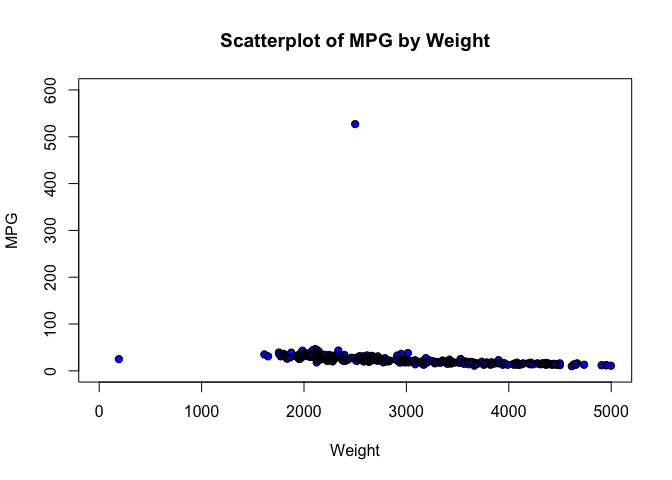
\includegraphics{RZone1_files/figure-latex/unnamed-chunk-16-1.pdf}

\hypertarget{create-a-scatterplot}{%
\subsubsection{CREATE A SCATTERPLOT}\label{create-a-scatterplot}}

\hypertarget{outliers-are-easily-spotted}{%
\paragraph{Outliers are easily
spotted}\label{outliers-are-easily-spotted}}

\begin{Shaded}
\begin{Highlighting}[]
  \KeywordTok{plot}\NormalTok{(cars2}\OperatorTok{$}\NormalTok{weight, cars2}\OperatorTok{$}\NormalTok{mpg,}
       \DataTypeTok{xlim =} \KeywordTok{c}\NormalTok{(}\DecValTok{0}\NormalTok{, }\DecValTok{5000}\NormalTok{), }\DataTypeTok{ylim =} \KeywordTok{c}\NormalTok{(}\DecValTok{0}\NormalTok{, }\DecValTok{600}\NormalTok{),}
       \DataTypeTok{xlab =} \StringTok{"Weight"}\NormalTok{, }\DataTypeTok{ylab =} \StringTok{"MPG"}\NormalTok{,}
       \DataTypeTok{main =} \StringTok{"Scatterplot of MPG by Weight"}\NormalTok{,}
       \DataTypeTok{type =} \StringTok{"p"}\NormalTok{, }\DataTypeTok{pch =} \DecValTok{16}\NormalTok{, }\DataTypeTok{col =} \StringTok{"blue"}\NormalTok{)}
  \CommentTok{#Add open black circles}
  \KeywordTok{points}\NormalTok{(cars2}\OperatorTok{$}\NormalTok{weight, cars2}\OperatorTok{$}\NormalTok{mpg,}
         \DataTypeTok{type =} \StringTok{"p"}\NormalTok{, }\DataTypeTok{col =} \StringTok{"black"}\NormalTok{)}
\end{Highlighting}
\end{Shaded}

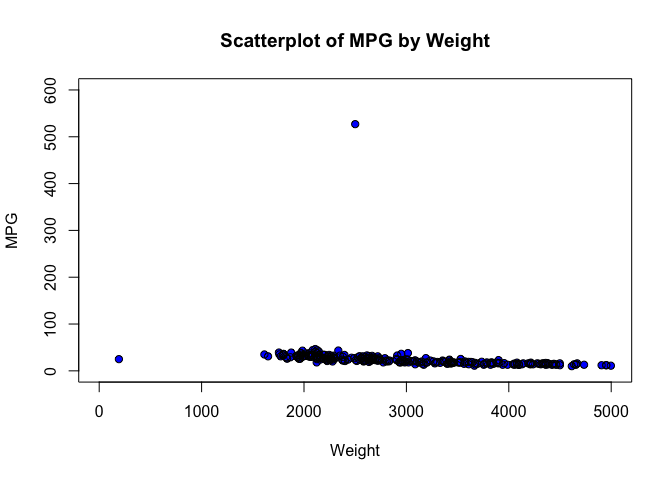
\includegraphics{RZone1_files/figure-latex/unnamed-chunk-17-1.pdf}

\hypertarget{descriptive-statistics}{%
\subsubsection{DESCRIPTIVE STATISTICS}\label{descriptive-statistics}}

\begin{Shaded}
\begin{Highlighting}[]
  \KeywordTok{mean}\NormalTok{(cars}\OperatorTok{$}\NormalTok{weight) }\CommentTok{# Mean}
\end{Highlighting}
\end{Shaded}

\begin{verbatim}
## [1] 3005.49
\end{verbatim}

\begin{Shaded}
\begin{Highlighting}[]
  \KeywordTok{median}\NormalTok{(cars}\OperatorTok{$}\NormalTok{weight) }\CommentTok{# Median}
\end{Highlighting}
\end{Shaded}

\begin{verbatim}
## [1] 2835
\end{verbatim}

\begin{Shaded}
\begin{Highlighting}[]
  \KeywordTok{length}\NormalTok{(cars}\OperatorTok{$}\NormalTok{weight) }\CommentTok{# Number of observations}
\end{Highlighting}
\end{Shaded}

\begin{verbatim}
## [1] 261
\end{verbatim}

\begin{Shaded}
\begin{Highlighting}[]
  \KeywordTok{sd}\NormalTok{(cars}\OperatorTok{$}\NormalTok{weight) }\CommentTok{# Standard deviation}
\end{Highlighting}
\end{Shaded}

\begin{verbatim}
## [1] 852.6456
\end{verbatim}

\begin{Shaded}
\begin{Highlighting}[]
  \KeywordTok{summary}\NormalTok{(cars}\OperatorTok{$}\NormalTok{weight) }\CommentTok{# Min, Q1, Median, Mean, Q3, Max}
\end{Highlighting}
\end{Shaded}

\begin{verbatim}
##    Min. 1st Qu.  Median    Mean 3rd Qu.    Max. 
##    1613    2246    2835    3005    3664    4997
\end{verbatim}

\hypertarget{transformations}{%
\subsubsection{TRANSFORMATIONS}\label{transformations}}

\hypertarget{outputs-suppressed-to-save-space-and-because-they-are-plotted-below.}{%
\paragraph{Outputs suppressed to save space and because they are plotted
below.}\label{outputs-suppressed-to-save-space-and-because-they-are-plotted-below.}}

\hypertarget{minmax-normalization-works-by-seeing-how-much-greater-the-field-value-is-than-the-minimum-value-minx-and-scaling-this-difference-by-the-range.}{%
\paragraph{Min--max normalization works by seeing how much greater the
field value is than the minimum value min(X), and scaling this
difference by the
range.}\label{minmax-normalization-works-by-seeing-how-much-greater-the-field-value-is-than-the-minimum-value-minx-and-scaling-this-difference-by-the-range.}}

\begin{Shaded}
\begin{Highlighting}[]
  \CommentTok{# Min-max normalization}
  \KeywordTok{summary}\NormalTok{(cars}\OperatorTok{$}\NormalTok{weight)}
\NormalTok{  mi <-}\StringTok{ }\KeywordTok{min}\NormalTok{(cars}\OperatorTok{$}\NormalTok{weight)}
\NormalTok{  ma <-}\StringTok{ }\KeywordTok{max}\NormalTok{(cars}\OperatorTok{$}\NormalTok{weight)}
\NormalTok{  minmax.weight <-}\StringTok{ }\NormalTok{(cars}\OperatorTok{$}\NormalTok{weight }\OperatorTok{-}\StringTok{ }\NormalTok{mi)}\OperatorTok{/}\NormalTok{(ma }\OperatorTok{-}\StringTok{ }\NormalTok{mi)}
\NormalTok{  minmax.weight}
\end{Highlighting}
\end{Shaded}

\hypertarget{z-score-standardization-which-is-very-widespread-in-the-world-of-statistical-analysis-works-by-taking-the-difference-between-the-field-value-and-the-field-mean-value-and-scaling-this-difference-by-the-sd-of-the-field-values.}{%
\paragraph{Z-score standardization, which is very widespread in the
world of statistical analysis, works by taking the difference between
the field value and the field mean value, and scaling this difference by
the SD of the field
values.}\label{z-score-standardization-which-is-very-widespread-in-the-world-of-statistical-analysis-works-by-taking-the-difference-between-the-field-value-and-the-field-mean-value-and-scaling-this-difference-by-the-sd-of-the-field-values.}}

\begin{Shaded}
\begin{Highlighting}[]
  \CommentTok{# Z-score standarization}
\NormalTok{  m <-}\StringTok{ }\KeywordTok{mean}\NormalTok{(cars}\OperatorTok{$}\NormalTok{weight); s <-}\StringTok{ }\KeywordTok{sd}\NormalTok{(cars}\OperatorTok{$}\NormalTok{weight)}
\NormalTok{  z.weight <-}\StringTok{ }\NormalTok{(cars}\OperatorTok{$}\NormalTok{weight }\OperatorTok{-}\StringTok{ }\NormalTok{m)}\OperatorTok{/}\NormalTok{s}
\NormalTok{  z.weight}
  \KeywordTok{length}\NormalTok{(cars}\OperatorTok{$}\NormalTok{weight)}
\end{Highlighting}
\end{Shaded}

\hypertarget{decimal-scaling-ensures-that-every-normalized-value-lies-between-1-and-1.}{%
\paragraph{Decimal scaling ensures that every normalized value lies
between −1 and
1.}\label{decimal-scaling-ensures-that-every-normalized-value-lies-between-1-and-1.}}

\begin{Shaded}
\begin{Highlighting}[]
  \CommentTok{# Decimal scaling}
  \KeywordTok{max}\NormalTok{(}\KeywordTok{abs}\NormalTok{(cars}\OperatorTok{$}\NormalTok{weight)) }\CommentTok{# 4 digits}
\NormalTok{  d.weight <-}\StringTok{ }\NormalTok{cars}\OperatorTok{$}\NormalTok{weight}\OperatorTok{/}\NormalTok{(}\DecValTok{10}\OperatorTok{^}\DecValTok{4}\NormalTok{); d.weight}
\end{Highlighting}
\end{Shaded}

\hypertarget{side-by-side-histograms}{%
\subsubsection{SIDE-BY-SIDE HISTOGRAMS}\label{side-by-side-histograms}}

\begin{Shaded}
\begin{Highlighting}[]
  \KeywordTok{par}\NormalTok{(}\DataTypeTok{mfrow =} \KeywordTok{c}\NormalTok{(}\DecValTok{1}\NormalTok{,}\DecValTok{2}\NormalTok{))}
  
  \CommentTok{# Create two histograms}
  \KeywordTok{hist}\NormalTok{(cars}\OperatorTok{$}\NormalTok{weight, }\DataTypeTok{breaks =} \DecValTok{20}\NormalTok{, }\DataTypeTok{xlim =} \KeywordTok{c}\NormalTok{(}\DecValTok{1000}\NormalTok{, }\DecValTok{5000}\NormalTok{),}
       \DataTypeTok{main =} \StringTok{"Histogram of Weight"}\NormalTok{, }\DataTypeTok{xlab =} \StringTok{"Weight"}\NormalTok{, }\DataTypeTok{ylab =} \StringTok{"Counts"}\NormalTok{)}
  \KeywordTok{box}\NormalTok{(}\DataTypeTok{which =} \StringTok{"plot"}\NormalTok{, }\DataTypeTok{lty =} \StringTok{"solid"}\NormalTok{, }\DataTypeTok{col =} \StringTok{"black"}\NormalTok{)}
  \KeywordTok{hist}\NormalTok{(z.weight, }\DataTypeTok{breaks =} \DecValTok{20}\NormalTok{, }\DataTypeTok{xlim =} \KeywordTok{c}\NormalTok{(}\OperatorTok{-}\DecValTok{2}\NormalTok{, }\DecValTok{3}\NormalTok{),}
       \DataTypeTok{main =} \StringTok{"Histogram of Z- score of Weight"}\NormalTok{,}
       \DataTypeTok{xlab =} \StringTok{"Z-score of Weight"}\NormalTok{, }\DataTypeTok{ylab =} \StringTok{"Counts"}\NormalTok{)}
  \KeywordTok{box}\NormalTok{(}\DataTypeTok{which =} \StringTok{"plot"}\NormalTok{, }\DataTypeTok{lty =} \StringTok{"solid"}\NormalTok{, }\DataTypeTok{col =} \StringTok{"black"}\NormalTok{)}
\end{Highlighting}
\end{Shaded}

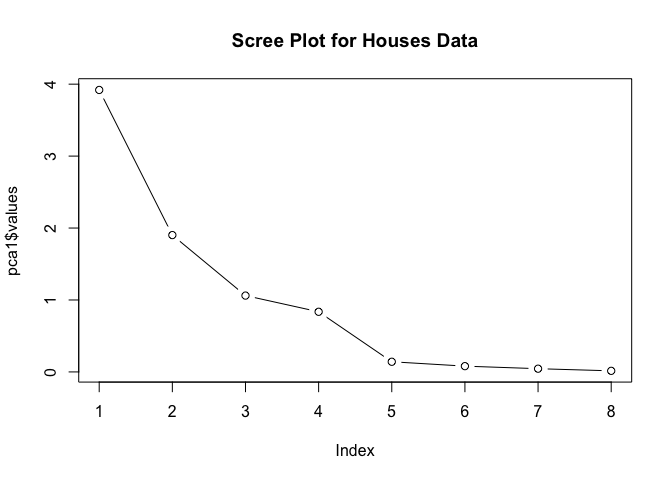
\includegraphics{RZone1_files/figure-latex/unnamed-chunk-22-1.pdf}

\hypertarget{skewness}{%
\subsubsection{SKEWNESS}\label{skewness}}

\hypertarget{skewness-describes-the-distance-between-the-median-and-the-mean.-positive-skewness-means-the-mean-is-greater-than-the-median-and-negative-skewness-means-the-mean-is-less-than-the-median.-zero-skewness-means-the-mean-is-equal-to-the-mode-when-the-data-is-unimodal.}{%
\paragraph{Skewness describes the distance between the median and the
mean. Positive skewness means the mean is greater than the median and
negative skewness means the mean is less than the median. Zero skewness
means the mean is equal to the mode (when the data is
unimodal).}\label{skewness-describes-the-distance-between-the-median-and-the-mean.-positive-skewness-means-the-mean-is-greater-than-the-median-and-negative-skewness-means-the-mean-is-less-than-the-median.-zero-skewness-means-the-mean-is-equal-to-the-mode-when-the-data-is-unimodal.}}

\begin{Shaded}
\begin{Highlighting}[]
\NormalTok{  (}\DecValTok{3}\OperatorTok{*}\NormalTok{(}\KeywordTok{mean}\NormalTok{(cars}\OperatorTok{$}\NormalTok{weight) }\OperatorTok{-}\StringTok{ }\KeywordTok{median}\NormalTok{(cars}\OperatorTok{$}\NormalTok{weight)))}\OperatorTok{/}\KeywordTok{sd}\NormalTok{(cars}\OperatorTok{$}\NormalTok{weight)}
\end{Highlighting}
\end{Shaded}

\begin{verbatim}
## [1] 0.5998638
\end{verbatim}

\begin{Shaded}
\begin{Highlighting}[]
\NormalTok{  (}\DecValTok{3}\OperatorTok{*}\NormalTok{(}\KeywordTok{mean}\NormalTok{(z.weight) }\OperatorTok{-}\StringTok{ }\KeywordTok{median}\NormalTok{(z.weight)))}\OperatorTok{/}\KeywordTok{sd}\NormalTok{(z.weight)}
\end{Highlighting}
\end{Shaded}

\begin{verbatim}
## [1] 0.5998638
\end{verbatim}

\hypertarget{transformations-for-normality}{%
\subsubsection{TRANSFORMATIONS FOR
NORMALITY}\label{transformations-for-normality}}

\hypertarget{these-transformations-attempt-to-reduce-skewness-and-make-the-data-more-normally-distributed.}{%
\paragraph{These transformations attempt to reduce skewness and make the
data ``more normally
distributed''.}\label{these-transformations-attempt-to-reduce-skewness-and-make-the-data-more-normally-distributed.}}

\begin{Shaded}
\begin{Highlighting}[]
\NormalTok{  sqrt.weight <-}\StringTok{ }\KeywordTok{sqrt}\NormalTok{(cars}\OperatorTok{$}\NormalTok{weight) }\CommentTok{# Square root}
\NormalTok{  sqrt.weight_skew <-}\StringTok{ }\NormalTok{(}\DecValTok{3}\OperatorTok{*}\NormalTok{(}\KeywordTok{mean}\NormalTok{(sqrt.weight) }\OperatorTok{-}\StringTok{ }\KeywordTok{median}\NormalTok{(sqrt.weight))) }\OperatorTok{/}\StringTok{ }\KeywordTok{sd}\NormalTok{(sqrt.weight)}
\NormalTok{  ln.weight <-}\StringTok{ }\KeywordTok{log}\NormalTok{(cars}\OperatorTok{$}\NormalTok{weight) }\CommentTok{# Natural log}
\NormalTok{  ln.weight_skew <-}\StringTok{ }\NormalTok{(}\DecValTok{3}\OperatorTok{*}\NormalTok{(}\KeywordTok{mean}\NormalTok{(ln.weight) }\OperatorTok{-}\StringTok{ }\KeywordTok{median}\NormalTok{(ln.weight))) }\OperatorTok{/}\StringTok{ }\KeywordTok{sd}\NormalTok{(ln.weight)}
\NormalTok{  invsqrt.weight <-}\StringTok{ }\DecValTok{1} \OperatorTok{/}\StringTok{ }\KeywordTok{sqrt}\NormalTok{(cars}\OperatorTok{$}\NormalTok{weight) }\CommentTok{# Inverse square root}
\NormalTok{  invsqrt.weight_skew <-}\StringTok{ }\NormalTok{(}\DecValTok{3}\OperatorTok{*}\NormalTok{(}\KeywordTok{mean}\NormalTok{(invsqrt.weight) }\OperatorTok{-}\StringTok{ }\KeywordTok{median}\NormalTok{(invsqrt.weight))) }\OperatorTok{/}\KeywordTok{sd}\NormalTok{(invsqrt.weight)}
\end{Highlighting}
\end{Shaded}

\hypertarget{histogram-with-normal-distribution-overlay}{%
\subsubsection{HISTOGRAM WITH NORMAL DISTRIBUTION
OVERLAY}\label{histogram-with-normal-distribution-overlay}}

\hypertarget{the-inverse-square-transformation-has-eliminated-skewness-but-it-is-still-not-normal.-this-is-clearly-seen-in-the-histogram-with-a-normal-overlay.}{%
\paragraph{The inverse square transformation has eliminated skewness,
but it is still not normal. This is clearly seen in the histogram with a
normal
overlay.}\label{the-inverse-square-transformation-has-eliminated-skewness-but-it-is-still-not-normal.-this-is-clearly-seen-in-the-histogram-with-a-normal-overlay.}}

\begin{Shaded}
\begin{Highlighting}[]
  \KeywordTok{par}\NormalTok{(}\DataTypeTok{mfrow=}\KeywordTok{c}\NormalTok{(}\DecValTok{1}\NormalTok{,}\DecValTok{1}\NormalTok{))}
\NormalTok{  x <-}\StringTok{ }\KeywordTok{rnorm}\NormalTok{(}\DecValTok{1000000}\NormalTok{, }\DataTypeTok{mean =} \KeywordTok{mean}\NormalTok{ (invsqrt.weight),}
             \DataTypeTok{sd =} \KeywordTok{sd}\NormalTok{(invsqrt.weight))}
  \KeywordTok{hist}\NormalTok{(invsqrt.weight, }\DataTypeTok{breaks =} \DecValTok{30}\NormalTok{, }\DataTypeTok{xlim =} \KeywordTok{c}\NormalTok{(}\FloatTok{0.0125}\NormalTok{, }\FloatTok{0.0275}\NormalTok{),}
       \DataTypeTok{col =} \StringTok{"lightblue"}\NormalTok{, }\DataTypeTok{prob =} \OtherTok{TRUE}\NormalTok{, }\DataTypeTok{border =} \StringTok{"black"}\NormalTok{,}
       \DataTypeTok{xlab =} \StringTok{"Inverse Square Root of Weight"}\NormalTok{,}
       \DataTypeTok{ylab =} \StringTok{"Counts"}\NormalTok{, }\DataTypeTok{main =} \StringTok{"Histogram of  Inverse Square Root of Weight"}\NormalTok{)}
  \KeywordTok{box}\NormalTok{(}\DataTypeTok{which =} \StringTok{"plot"}\NormalTok{, }\DataTypeTok{lty =} \StringTok{"solid"}\NormalTok{, }\DataTypeTok{col=}\StringTok{"black"}\NormalTok{)}
  
  \CommentTok{# Overlay with  Normal density}
  \KeywordTok{lines}\NormalTok{(}\KeywordTok{density}\NormalTok{(x), }\DataTypeTok{col =} \StringTok{"red"}\NormalTok{)}
\end{Highlighting}
\end{Shaded}

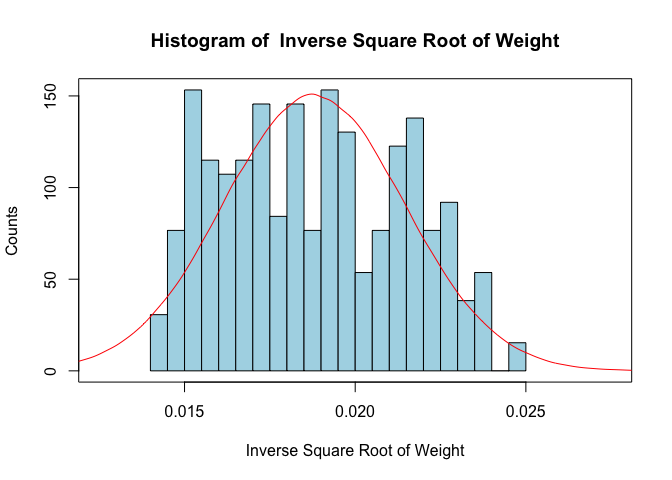
\includegraphics{RZone1_files/figure-latex/unnamed-chunk-25-1.pdf}

\hypertarget{normal-q-q-plot}{%
\subsubsection{NORMAL Q-Q PLOT}\label{normal-q-q-plot}}

\hypertarget{the-q-q-plot-shows-that-our-data-shows-systematic-deviations-from-non-normality.}{%
\paragraph{The Q-Q plot shows that our data shows systematic deviations
from
non-normality.}\label{the-q-q-plot-shows-that-our-data-shows-systematic-deviations-from-non-normality.}}

\begin{Shaded}
\begin{Highlighting}[]
  \KeywordTok{qqnorm}\NormalTok{(invsqrt.weight, }\DataTypeTok{datax =} \OtherTok{TRUE}\NormalTok{, }\DataTypeTok{col =} \StringTok{"red"}\NormalTok{, }\DataTypeTok{ylim =} \KeywordTok{c}\NormalTok{(}\FloatTok{0.01}\NormalTok{, }\FloatTok{0.03}\NormalTok{),}
         \DataTypeTok{main =} \StringTok{"Normal Q-Q Plot of Inverse Square Root of Weight"}\NormalTok{)}
  \KeywordTok{qqline}\NormalTok{(invsqrt.weight, }\DataTypeTok{col =} \StringTok{"blue"}\NormalTok{, }\DataTypeTok{datax =} \OtherTok{TRUE}\NormalTok{)}
\end{Highlighting}
\end{Shaded}

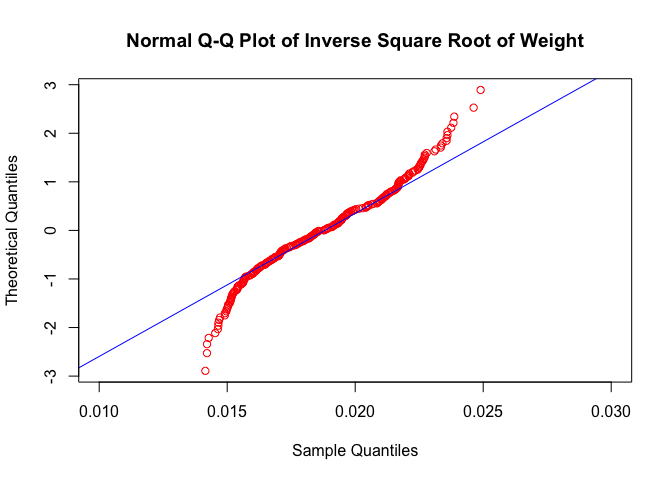
\includegraphics{RZone1_files/figure-latex/unnamed-chunk-26-1.pdf}

\hypertarget{de-transform-data}{%
\subsubsection{DE-TRANSFORM DATA}\label{de-transform-data}}

\begin{Shaded}
\begin{Highlighting}[]
  \CommentTok{# Transform x using y = 1 / sqrt(x)}
\NormalTok{  x <-}\StringTok{ }\NormalTok{cars}\OperatorTok{$}\NormalTok{weight[}\DecValTok{1}\NormalTok{]; y <-}\StringTok{ }\DecValTok{1} \OperatorTok{/}\StringTok{ }\KeywordTok{sqrt}\NormalTok{(x)}
  
  \CommentTok{# Detransform x using x = 1 / (y)^2}
\NormalTok{  detransformedx <-}\StringTok{ }\DecValTok{1} \OperatorTok{/}\StringTok{ }\NormalTok{y}\OperatorTok{^}\DecValTok{2}
\NormalTok{  x; y; detransformedx}
\end{Highlighting}
\end{Shaded}

\begin{verbatim}
## [1] 4209
\end{verbatim}

\begin{verbatim}
## [1] 0.01541383
\end{verbatim}

\begin{verbatim}
## [1] 4209
\end{verbatim}

\hypertarget{create-indicator-variables}{%
\subsubsection{CREATE INDICATOR
VARIABLES}\label{create-indicator-variables}}

\begin{Shaded}
\begin{Highlighting}[]
\NormalTok{  north_flag <-}\StringTok{ }\NormalTok{east_flag <-}\StringTok{ }\NormalTok{south_flag <-}\StringTok{ }\KeywordTok{c}\NormalTok{(}\KeywordTok{rep}\NormalTok{(}\OtherTok{NA}\NormalTok{, }\DecValTok{10}\NormalTok{))}
\NormalTok{  region <-}\StringTok{ }\KeywordTok{c}\NormalTok{(}\KeywordTok{rep}\NormalTok{(}\KeywordTok{c}\NormalTok{(}\StringTok{"north"}\NormalTok{, }\StringTok{"south"}\NormalTok{, }\StringTok{"east"}\NormalTok{, }\StringTok{"west"}\NormalTok{),}\DecValTok{2}\NormalTok{), }\StringTok{"north"}\NormalTok{, }\StringTok{"south"}\NormalTok{)}
  
  \CommentTok{# Change the region variable to indicators}
  \ControlFlowTok{for}\NormalTok{ (i }\ControlFlowTok{in} \DecValTok{1}\OperatorTok{:}\KeywordTok{length}\NormalTok{(region)) \{}
    \ControlFlowTok{if}\NormalTok{(region[i] }\OperatorTok{==}\StringTok{ "north"}\NormalTok{) north_flag[i] =}\StringTok{ }\DecValTok{1}
    \ControlFlowTok{else}\NormalTok{ north_flag[i] =}\StringTok{ }\DecValTok{0}
    \ControlFlowTok{if}\NormalTok{(region[i] }\OperatorTok{==}\StringTok{ "east"}\NormalTok{) east_flag[i] =}\StringTok{ }\DecValTok{1}
    \ControlFlowTok{else}\NormalTok{ east_flag[i] =}\StringTok{ }\DecValTok{0}
    \ControlFlowTok{if}\NormalTok{(region[i] }\OperatorTok{==}\StringTok{ "south"}\NormalTok{) south_flag[i] =}\StringTok{ }\DecValTok{1}
    \ControlFlowTok{else}\NormalTok{ south_flag[i] =}\StringTok{ }\DecValTok{0}
\NormalTok{  \}}
\NormalTok{  north_flag; east_flag; south_flag}
\end{Highlighting}
\end{Shaded}

\begin{verbatim}
##  [1] 1 0 0 0 1 0 0 0 1 0
\end{verbatim}

\begin{verbatim}
##  [1] 0 0 1 0 0 0 1 0 0 0
\end{verbatim}

\begin{verbatim}
##  [1] 0 1 0 0 0 1 0 0 0 1
\end{verbatim}

\begin{Shaded}
\begin{Highlighting}[]
\CommentTok{### INDEX FIELDS}
  \CommentTok{# Data frames have an index field;}
  \CommentTok{# the left-most column}
\NormalTok{  cars}
\end{Highlighting}
\end{Shaded}

\begin{verbatim}
##      mpg cylinders cubicinches  hp weightlbs time.to.60 year    brand
## 1   14.0         8         350 165      4209         12 1972      US.
## 2   31.9         4          89  71      1925         14 1980  Europe.
## 3   17.0         8         302 140      3449         11 1971      US.
## 4   15.0         8         400 150      3761         10 1971      US.
## 5   30.5         4          98  63      2051         17 1978      US.
## 6   23.0         8         350 125      3900         17 1980      US.
## 7   13.0         8         351 158      4363         13 1974      US.
## 8   14.0         8         440 215      4312          9 1971      US.
## 9   25.4         5         183  77      3530         20 1980  Europe.
## 10  37.7         4          89  62      2050         17 1982   Japan.
## 11  34.0         4         108  70      2245         17 1983   Japan.
## 12  34.3         4          97  78      2188         16 1981  Europe.
## 13  16.0         8         302 140      4141         14 1975      US.
## 14  11.0         8         350 180      3664         11 1974      US.
## 15  19.1         6         225  90      3381         19 1981      US.
## 16  16.9         8         350 155      4360         15 1980      US.
## 17  31.8         4          85  65      2020         19 1980   Japan.
## 18  16.0         8         304 150      3433         12 1971      US.
## 19  24.0         4         113  95      2278         16 1973   Japan.
## 20  24.0         4         107  90      2430         15 1971  Europe.
## 21  37.2         4          86  65      2019         16 1981   Japan.
## 22  21.5         4         121 110      2600         13 1978  Europe.
## 23  24.0         6         200  81      3012         18 1977      US.
## 24  15.5         8         351 142      4054         14 1980      US.
## 25  38.1         4          89  60      1968         19 1981   Japan.
## 26  33.0         4          91  53      1795         17 1977   Japan.
## 27  31.0         4          71  65      1773         19 1972   Japan.
## 28  14.0         8         351 148      4657         14 1976      US.
## 29  18.0         6         250  78      3574         21 1977      US.
## 30  29.9         4          98  65      2380         21 1982      US.
## 31  27.0         4          97  88      2130         15 1971   Japan.
## 32  16.0         6         250 100      3278         18 1974      US.
## 33  23.0         4         120  97      2506         15 1973   Japan.
## 34  21.0         6         199  90      2648         15 1971      US.
## 35  30.0         4          97  67      1985         16 1978   Japan.
## 36  22.4         6         231 110      3415         16 1982      US.
## 37  26.0         4          97  46      1835         21 1971  Europe.
## 38  21.5         3          80 110      2720         14 1978   Japan.
## 39  16.5         8         351 138      3955         13 1980      US.
## 40  20.2         6         232  90      3265         18 1980      US.
## 41  16.0         6         250 105      3897         19 1976      US.
## 42  14.0         8         302 140      4638         16 1975      US.
## 43  18.5         6         250 110      3645         16 1977      US.
## 44  17.5         6         250 110      3520         16 1978      US.
## 45  14.0         8         455 225      3086         10 1971      US.
## 46  31.6         4         120  74      2635         18 1982   Japan.
## 47  13.0         8         318 150      3755         14 1977      US.
## 48  22.0         4         122  86      2395         16 1973      US.
## 49  29.0         4          97  78      1940         15 1978  Europe.
## 50  20.2         6         200  88      3060         17 1982      US.
## 51  13.0         8         400 150      4464         12 1974      US.
## 52  27.2         4         141  71      3190         25 1980  Europe.
## 53  14.0         8         340 160      3609          8 1971      US.
## 54  24.0         4         116  75      2158         16 1974  Europe.
## 55  16.5         8         350 180      4380         12 1977      US.
## 56  16.0         8         400 230      4278         10 1974      US.
## 57  19.0         6         156 108      2930         16 1977   Japan.
## 58  33.5         4          98  83      2075         16 1978      US.
## 59  29.0         4          90  70      1937         14 1977  Europe.
## 60  13.0         8         360 175      3821         11 1974      US.
## 61  18.0         6         232 100      2945         16 1974      US.
## 62  22.0         4         108  94      2379         17 1974   Japan.
## 63  32.7         6         168 132      2910         11 1981   Japan.
## 64  46.6         4          86  65      2110         18 1981   Japan.
## 65  14.0         8         318 150      4237         15 1974      US.
## 66  18.5         6         250  98      3525         19 1978      US.
## 67  26.0         4          97  46      1950         21 1974  Europe.
## 68  32.0         4          91  67      1965         16 1983   Japan.
## 69  29.5         4          97  71      1825         12 1977  Europe.
## 70  17.5         8         305 145      3880         13 1978      US.
## 71  20.0         6         198  95      3102         17 1975      US.
## 72  27.0         4         112  88      2640         19 1983      US.
## 73  28.0         4          97  92      2288         17 1973   Japan.
## 74  24.0         4         119  97      2545         17 1976   Japan.
## 75  29.0         4          98  83      2219         17 1975  Europe.
## 76  38.0         6         262  85      3015         17 1983      US.
## 77  22.5         6         232  90      3085         18 1977      US.
## 78  21.1         4         134  95      2515         15 1979   Japan.
## 79  26.0         4          98  90      2265         16 1974  Europe.
## 80  32.4         4         108  75      2350         17 1982   Japan.
## 81  15.5         8         400 190      4325         12 1978      US.
## 82  12.0         8         429 198      4952         12 1974      US.
## 83  19.2         8         305 145      3425         13 1979      US.
## 84  23.0         4         115  95      2694         15 1976  Europe.
## 85  25.0         4         116  81      2220         17 1977  Europe.
## 86  35.0         4          72  69      1613         18 1972   Japan.
## 87  18.0         6         199  97      2774         16 1971      US.
## 88  17.6         6         225  85      3465         17 1982      US.
## 89  28.0         4          90  75      2125         15 1975      US.
## 90  31.0         4         119  82      2720         19 1983      US.
## 91  34.1         4          86  65      1975         15 1980   Japan.
## 92  27.2         4         119  97      2300         15 1979   Japan.
## 93  13.0         8         350 175      4100         13 1974      US.
## 94  17.0         6         250 100      3329         16 1972      US.
## 95  26.0         4          98  79      2255         18 1977      US.
## 96  17.0         6         231 110      3907         21 1976      US.
## 97  12.0         8         350 180      4499         13 1974      US.
## 98  18.0         6         250  88      3139         15 1972      US.
## 99  18.2         8         318 135      3830         15 1980      US.
## 100 16.0         6         250 100      3781         17 1975      US.
## 101 11.0         8         400 150      4997         14 1974      US.
## 102 12.0         8         400 167      4906         13 1974      US.
## 103 25.0         4          98  80      2126         17 1973      US.
## 104 34.2         4         105  70      2200         13 1980      US.
## 105 32.2         4         108  75      2265         15 1981   Japan.
## 106 26.6         4         151  84      2635         16 1982      US.
## 107 43.4         4          90  48      2335         24 1981  Europe.
## 108 30.0         4          88  76      2065         15 1972  Europe.
## 109 25.0         4         121 115      2671         14 1976  Europe.
## 110 18.0         8         307 130      3504         12 1971      US.
## 111 20.0         4          97  88      2279         19 1974   Japan.
## 112 18.0         4         121 112      2933         15 1973  Europe.
## 113 16.0         8         351 149      4335         15 1978      US.
## 114 33.0         4          91  53      1795         18 1976   Japan.
## 115 37.3         4          91  69      2130         15 1980  Europe.
## 116 18.0         6         225  95      3785         19 1976      US.
## 117 24.5         4         151  88      2740         16 1978      US.
## 118 21.0         6         231 110      3039         15 1976      US.
## 119 34.4         4          98  65      2045         16 1982      US.
## 120 15.0         8         429 198      4341         10 1971      US.
## 121 27.0         4         101  83      2202         15 1977  Europe.
## 122 26.0         4          79  67      1963         16 1975  Europe.
## 123 16.0         8         400 170      4668         12 1976      US.
## 124 23.2         4         156 105      2745         17 1979      US.
## 125 27.0         4          97  60      1834         19 1972  Europe.
## 126 26.5         4         140  72      2565         14 1977      US.
## 127 13.0         8         360 170      4654         13 1974      US.
## 128 30.9         4         105  75      2230         15 1979      US.
## 129 20.0         4         114  91      2582         14 1974  Europe.
## 130 36.1         4          98  66      1800         14 1979      US.
## 131 26.0         4          97  78      2300         15 1975  Europe.
## 132 28.0         4         151  90      2678         17 1981      US.
## 133 12.0         8         455 225      4951         11 1974      US.
## 134 17.0         8         304 150      3672         12 1973      US.
## 135 15.0         8         350 145      4440         14 1976      US.
## 136 16.0         8         318 150      4190         13 1977      US.
## 137 26.0         4          91  70      1955         21 1972      US.
## 138 13.0         8         302 129      3169         12 1976      US.
## 139 22.0         4         121  98      2945         15 1976  Europe.
## 140 21.0         4         120  87      2979         20 1973  Europe.
## 141 26.8         6         173 115      2700         13 1980      US.
## 142 29.0         4          97  75      2171         16 1976   Japan.
## 143 32.0         4         144  96      2665         14 1983   Japan.
## 144 35.1         4          81  60      1760         16 1982   Japan.
## 145 19.2         8         267 125      3605         15 1980      US.
## 146 23.0         4         120  88      2957         17 1976  Europe.
## 147 20.6         6         225 110      3360         17 1980      US.
## 148 27.0         4         151  90      2735         18 1983      US.
## 149 15.0         8         350 165      3693         12 1971      US.
## 150 18.1         8         302 139      3205         11 1979      US.
## 151 31.3         4         120  75      2542         18 1981   Japan.
## 152 27.5         4         134  95      2560         14 1979   Japan.
## 153 14.0         8         455 225      4425         10 1971      US.
## 154 15.0         6         250  72      3158         20 1976      US.
## 155 28.0         4         107  86      2464         16 1977  Europe.
## 156 19.0         6         250  88      3302         16 1972      US.
## 157 18.0         3          70  90      2124         14 1974   Japan.
## 158 29.5         4          98  68      2135         17 1979   Japan.
## 159 19.0         6         232 100      2634         13 1972      US.
## 160 16.2         6         163 133      3410         16 1979  Europe.
## 161 24.3         4         151  90      3003         20 1981      US.
## 162 17.5         8         318 140      4080         14 1979      US.
## 163 18.0         6         171  97      2984         15 1976      US.
## 164 23.0         6         198  95      2904         16 1974      US.
## 165 23.0         4          97  54      2254         24 1973  Europe.
## 166 19.9         8         260 110      3365         16 1979      US.
## 167 16.0         6         225 105      3439         16 1972      US.
## 168 26.0         4         156  92      2585         15 1983      US.
## 169 20.0         6         156 122      2807         14 1974   Japan.
## 170 38.0         4         105  63      2125         15 1983      US.
## 171 32.4         4         107  72      2290         17 1981   Japan.
## 172 20.3         5         131 103      2830         16 1979  Europe.
## 173 29.0         4          68  49      1867         20 1974  Europe.
## 174 31.0         4         112  85      2575         16 1983      US.
## 175 21.0         4         122  86      2226         17 1973      US.
## 176 26.0         4          96  69      2189         18 1973  Europe.
## 177 14.0         8         400 175      4385         12 1973      US.
## 178 14.0         8         304 150      3672         12 1974      US.
## 179 20.2         8         302 139      3570         13 1979      US.
## 180 31.5         4          98  68      2045         19 1978   Japan.
## 181 19.8         6         200  85      2990         18 1980      US.
## 182 33.8         4          97  67      2145         18 1981   Japan.
## 183 17.5         8         305 140      4215         13 1977      US.
## 184 18.0         8         318 150      3436         11 1971      US.
## 185 34.0         4         112  88      2395         18 1983      US.
## 186 20.8         6         200  85      3070         17 1979      US.
## 187 18.0         6         250 105      3459         16 1976      US.
## 188 13.0         8         318 150      3940         13 1977      US.
## 189 14.0         8         351 153      4129         13 1973      US.
## 190 13.0         8         440 215      4735         11 1974      US.
## 191 25.8         4         156  92      2620         14 1982      US.
## 192 28.4         4         151  90      2670         16 1980      US.
## 193 13.0         8         400 190      4422         13 1973      US.
## 194 15.0         8         350 145      4082         13 1974      US.
## 195 14.0         8         318 150      4077         14 1973      US.
## 196 41.5         4          98  76      2144         15 1981  Europe.
## 197 27.2         4         135  84      2490         16 1982      US.
## 198 43.1         4          90  48      1985         22 1979  Europe.
## 199 29.0         4          90  70      1937         14 1976  Europe.
## 200 33.5         4          85  70      1945         17 1978   Japan.
## 201 26.0         4         116  75      2246         14 1975  Europe.
## 202 23.0         4         140  83      2639         17 1976      US.
## 203 23.9         8         260  90      3420         22 1980      US.
## 204 19.0         6         225 100      3630         18 1978      US.
## 205 21.0         4         140  72      2401         20 1974      US.
## 206 15.0         8         390 190      3850          9 1971      US.
## 207 40.8         4          85  65      2110         19 1981   Japan.
## 208 18.0         6         250  88      3021         17 1974      US.
## 209 13.0         8         307 130      4098         14 1973      US.
## 210 25.4         6         168 116      2900         13 1982   Japan.
## 211 22.0         6         146  97      2815         15 1978   Japan.
## 212 17.7         6         231 165      3445         13 1979      US.
## 213 39.1         4          79  58      1755         17 1982   Japan.
## 214 30.0         4          79  70      2074         20 1972  Europe.
## 215 22.0         6         225 100      3233         15 1977      US.
## 216 32.9         4         119 100      2615         15 1982   Japan.
## 217 37.0         4          85  65      1975         19 1982   Japan.
## 218 14.5         8         351 152      4215         13 1977      US.
## 219 28.8         6         173 115      2595         11 1980      US.
## 220 15.0         8         302 130      4295         15 1978      US.
## 221 17.5         6         258  95      3193         18 1977      US.
## 222 21.6         4         121 115      2795         16 1979  Europe.
## 223 14.0         8         318 150      4457         14 1975      US.
## 224 16.5         6         168 120      3820         17 1977  Europe.
## 225 14.0         8         302 137      4042         15 1974      US.
## 226 32.0         4          83  61      2003         19 1975   Japan.
## 227 10.0         8         360 215      4615         14 1971      US.
## 228 31.0         4          76  52      1649         17 1975   Japan.
## 229 21.0         6         200  85      2587         16 1971      US.
## 230 27.0         4         140  86      2790         16 1983      US.
## 231 15.0         8         383 170      3563         10 1971      US.
## 232 28.0         4         120  79      2625         19 1983      US.
## 233 23.0         4         140  78      2592         19 1976      US.
## 234 16.0         8         318 150      4498         15 1976      US.
## 235 20.0         4         130 102      3150         16 1977  Europe.
## 236 44.0         4          97  52      2130         25 1983  Europe.
## 237 14.0         8         318 150      4096         13 1972      US.
## 238 20.2         6         200  85      2965         16 1979      US.
## 239 39.0         4          86  64      1875         16 1982      US.
## 240 23.0         4         122  86      2220         14 1972      US.
## 241 13.0         8         350 145      4055         12 1977      US.
## 242 18.0         6         225 105      3121         17 1974      US.
## 243 16.0         8         400 180      4220         11 1978      US.
## 244 25.0         4         110  87      2672         18 1971  Europe.
## 245 14.0         8         454 220      4354          9 1971      US.
## 246 15.0         8         318 150      3399         11 1974      US.
## 247 19.4         8         318 140      3735         13 1979      US.
## 248 44.3         4          90  48      2085         22 1981  Europe.
## 249 28.0         4          97  75      2155         16 1977   Japan.
## 250 29.0         4         135  84      2525         16 1983      US.
## 251 32.1         4          98  70      2120         16 1981      US.
## 252 24.0         4         121 110      2660         14 1974  Europe.
## 253 36.4         5         121  67      2950         20 1981  Europe.
## 254 13.0         8         350 145      3988         13 1974      US.
## 255 23.5         6         173 110      2725         13 1982      US.
## 256 24.0         4         113  95      2372         15 1971   Japan.
## 257 17.0         8         305 130      3840         15 1980      US.
## 258 36.1         4          91  60      1800         16 1979   Japan.
## 259 22.0         6         232 112      2835         15 1983      US.
## 260 18.0         6         232 100      3288         16 1972      US.
## 261 22.0         6         250 105      3353         15 1977      US.
\end{verbatim}

\begin{Shaded}
\begin{Highlighting}[]
\NormalTok{  cars[}\KeywordTok{order}\NormalTok{(cars}\OperatorTok{$}\NormalTok{mpg),]}
\end{Highlighting}
\end{Shaded}

\begin{verbatim}
##      mpg cylinders cubicinches  hp weightlbs time.to.60 year    brand
## 227 10.0         8         360 215      4615         14 1971      US.
## 14  11.0         8         350 180      3664         11 1974      US.
## 101 11.0         8         400 150      4997         14 1974      US.
## 82  12.0         8         429 198      4952         12 1974      US.
## 97  12.0         8         350 180      4499         13 1974      US.
## 102 12.0         8         400 167      4906         13 1974      US.
## 133 12.0         8         455 225      4951         11 1974      US.
## 7   13.0         8         351 158      4363         13 1974      US.
## 47  13.0         8         318 150      3755         14 1977      US.
## 51  13.0         8         400 150      4464         12 1974      US.
## 60  13.0         8         360 175      3821         11 1974      US.
## 93  13.0         8         350 175      4100         13 1974      US.
## 127 13.0         8         360 170      4654         13 1974      US.
## 138 13.0         8         302 129      3169         12 1976      US.
## 188 13.0         8         318 150      3940         13 1977      US.
## 190 13.0         8         440 215      4735         11 1974      US.
## 193 13.0         8         400 190      4422         13 1973      US.
## 209 13.0         8         307 130      4098         14 1973      US.
## 241 13.0         8         350 145      4055         12 1977      US.
## 254 13.0         8         350 145      3988         13 1974      US.
## 1   14.0         8         350 165      4209         12 1972      US.
## 8   14.0         8         440 215      4312          9 1971      US.
## 28  14.0         8         351 148      4657         14 1976      US.
## 42  14.0         8         302 140      4638         16 1975      US.
## 45  14.0         8         455 225      3086         10 1971      US.
## 53  14.0         8         340 160      3609          8 1971      US.
## 65  14.0         8         318 150      4237         15 1974      US.
## 153 14.0         8         455 225      4425         10 1971      US.
## 177 14.0         8         400 175      4385         12 1973      US.
## 178 14.0         8         304 150      3672         12 1974      US.
## 189 14.0         8         351 153      4129         13 1973      US.
## 195 14.0         8         318 150      4077         14 1973      US.
## 223 14.0         8         318 150      4457         14 1975      US.
## 225 14.0         8         302 137      4042         15 1974      US.
## 237 14.0         8         318 150      4096         13 1972      US.
## 245 14.0         8         454 220      4354          9 1971      US.
## 218 14.5         8         351 152      4215         13 1977      US.
## 4   15.0         8         400 150      3761         10 1971      US.
## 120 15.0         8         429 198      4341         10 1971      US.
## 135 15.0         8         350 145      4440         14 1976      US.
## 149 15.0         8         350 165      3693         12 1971      US.
## 154 15.0         6         250  72      3158         20 1976      US.
## 194 15.0         8         350 145      4082         13 1974      US.
## 206 15.0         8         390 190      3850          9 1971      US.
## 220 15.0         8         302 130      4295         15 1978      US.
## 231 15.0         8         383 170      3563         10 1971      US.
## 246 15.0         8         318 150      3399         11 1974      US.
## 24  15.5         8         351 142      4054         14 1980      US.
## 81  15.5         8         400 190      4325         12 1978      US.
## 13  16.0         8         302 140      4141         14 1975      US.
## 18  16.0         8         304 150      3433         12 1971      US.
## 32  16.0         6         250 100      3278         18 1974      US.
## 41  16.0         6         250 105      3897         19 1976      US.
## 56  16.0         8         400 230      4278         10 1974      US.
## 100 16.0         6         250 100      3781         17 1975      US.
## 113 16.0         8         351 149      4335         15 1978      US.
## 123 16.0         8         400 170      4668         12 1976      US.
## 136 16.0         8         318 150      4190         13 1977      US.
## 167 16.0         6         225 105      3439         16 1972      US.
## 234 16.0         8         318 150      4498         15 1976      US.
## 243 16.0         8         400 180      4220         11 1978      US.
## 160 16.2         6         163 133      3410         16 1979  Europe.
## 39  16.5         8         351 138      3955         13 1980      US.
## 55  16.5         8         350 180      4380         12 1977      US.
## 224 16.5         6         168 120      3820         17 1977  Europe.
## 16  16.9         8         350 155      4360         15 1980      US.
## 3   17.0         8         302 140      3449         11 1971      US.
## 94  17.0         6         250 100      3329         16 1972      US.
## 96  17.0         6         231 110      3907         21 1976      US.
## 134 17.0         8         304 150      3672         12 1973      US.
## 257 17.0         8         305 130      3840         15 1980      US.
## 44  17.5         6         250 110      3520         16 1978      US.
## 70  17.5         8         305 145      3880         13 1978      US.
## 162 17.5         8         318 140      4080         14 1979      US.
## 183 17.5         8         305 140      4215         13 1977      US.
## 221 17.5         6         258  95      3193         18 1977      US.
## 88  17.6         6         225  85      3465         17 1982      US.
## 212 17.7         6         231 165      3445         13 1979      US.
## 29  18.0         6         250  78      3574         21 1977      US.
## 61  18.0         6         232 100      2945         16 1974      US.
## 87  18.0         6         199  97      2774         16 1971      US.
## 98  18.0         6         250  88      3139         15 1972      US.
## 110 18.0         8         307 130      3504         12 1971      US.
## 112 18.0         4         121 112      2933         15 1973  Europe.
## 116 18.0         6         225  95      3785         19 1976      US.
## 157 18.0         3          70  90      2124         14 1974   Japan.
## 163 18.0         6         171  97      2984         15 1976      US.
## 184 18.0         8         318 150      3436         11 1971      US.
## 187 18.0         6         250 105      3459         16 1976      US.
## 208 18.0         6         250  88      3021         17 1974      US.
## 242 18.0         6         225 105      3121         17 1974      US.
## 260 18.0         6         232 100      3288         16 1972      US.
## 150 18.1         8         302 139      3205         11 1979      US.
## 99  18.2         8         318 135      3830         15 1980      US.
## 43  18.5         6         250 110      3645         16 1977      US.
## 66  18.5         6         250  98      3525         19 1978      US.
## 57  19.0         6         156 108      2930         16 1977   Japan.
## 156 19.0         6         250  88      3302         16 1972      US.
## 159 19.0         6         232 100      2634         13 1972      US.
## 204 19.0         6         225 100      3630         18 1978      US.
## 15  19.1         6         225  90      3381         19 1981      US.
## 83  19.2         8         305 145      3425         13 1979      US.
## 145 19.2         8         267 125      3605         15 1980      US.
## 247 19.4         8         318 140      3735         13 1979      US.
## 181 19.8         6         200  85      2990         18 1980      US.
## 166 19.9         8         260 110      3365         16 1979      US.
## 71  20.0         6         198  95      3102         17 1975      US.
## 111 20.0         4          97  88      2279         19 1974   Japan.
## 129 20.0         4         114  91      2582         14 1974  Europe.
## 169 20.0         6         156 122      2807         14 1974   Japan.
## 235 20.0         4         130 102      3150         16 1977  Europe.
## 40  20.2         6         232  90      3265         18 1980      US.
## 50  20.2         6         200  88      3060         17 1982      US.
## 179 20.2         8         302 139      3570         13 1979      US.
## 238 20.2         6         200  85      2965         16 1979      US.
## 172 20.3         5         131 103      2830         16 1979  Europe.
## 147 20.6         6         225 110      3360         17 1980      US.
## 186 20.8         6         200  85      3070         17 1979      US.
## 34  21.0         6         199  90      2648         15 1971      US.
## 118 21.0         6         231 110      3039         15 1976      US.
## 140 21.0         4         120  87      2979         20 1973  Europe.
## 175 21.0         4         122  86      2226         17 1973      US.
## 205 21.0         4         140  72      2401         20 1974      US.
## 229 21.0         6         200  85      2587         16 1971      US.
## 78  21.1         4         134  95      2515         15 1979   Japan.
## 22  21.5         4         121 110      2600         13 1978  Europe.
## 38  21.5         3          80 110      2720         14 1978   Japan.
## 222 21.6         4         121 115      2795         16 1979  Europe.
## 48  22.0         4         122  86      2395         16 1973      US.
## 62  22.0         4         108  94      2379         17 1974   Japan.
## 139 22.0         4         121  98      2945         15 1976  Europe.
## 211 22.0         6         146  97      2815         15 1978   Japan.
## 215 22.0         6         225 100      3233         15 1977      US.
## 259 22.0         6         232 112      2835         15 1983      US.
## 261 22.0         6         250 105      3353         15 1977      US.
## 36  22.4         6         231 110      3415         16 1982      US.
## 77  22.5         6         232  90      3085         18 1977      US.
## 6   23.0         8         350 125      3900         17 1980      US.
## 33  23.0         4         120  97      2506         15 1973   Japan.
## 84  23.0         4         115  95      2694         15 1976  Europe.
## 146 23.0         4         120  88      2957         17 1976  Europe.
## 164 23.0         6         198  95      2904         16 1974      US.
## 165 23.0         4          97  54      2254         24 1973  Europe.
## 202 23.0         4         140  83      2639         17 1976      US.
## 233 23.0         4         140  78      2592         19 1976      US.
## 240 23.0         4         122  86      2220         14 1972      US.
## 124 23.2         4         156 105      2745         17 1979      US.
## 255 23.5         6         173 110      2725         13 1982      US.
## 203 23.9         8         260  90      3420         22 1980      US.
## 19  24.0         4         113  95      2278         16 1973   Japan.
## 20  24.0         4         107  90      2430         15 1971  Europe.
## 23  24.0         6         200  81      3012         18 1977      US.
## 54  24.0         4         116  75      2158         16 1974  Europe.
## 74  24.0         4         119  97      2545         17 1976   Japan.
## 252 24.0         4         121 110      2660         14 1974  Europe.
## 256 24.0         4         113  95      2372         15 1971   Japan.
## 161 24.3         4         151  90      3003         20 1981      US.
## 117 24.5         4         151  88      2740         16 1978      US.
## 85  25.0         4         116  81      2220         17 1977  Europe.
## 103 25.0         4          98  80      2126         17 1973      US.
## 109 25.0         4         121 115      2671         14 1976  Europe.
## 244 25.0         4         110  87      2672         18 1971  Europe.
## 9   25.4         5         183  77      3530         20 1980  Europe.
## 210 25.4         6         168 116      2900         13 1982   Japan.
## 191 25.8         4         156  92      2620         14 1982      US.
## 37  26.0         4          97  46      1835         21 1971  Europe.
## 67  26.0         4          97  46      1950         21 1974  Europe.
## 79  26.0         4          98  90      2265         16 1974  Europe.
## 95  26.0         4          98  79      2255         18 1977      US.
## 122 26.0         4          79  67      1963         16 1975  Europe.
## 131 26.0         4          97  78      2300         15 1975  Europe.
## 137 26.0         4          91  70      1955         21 1972      US.
## 168 26.0         4         156  92      2585         15 1983      US.
## 176 26.0         4          96  69      2189         18 1973  Europe.
## 201 26.0         4         116  75      2246         14 1975  Europe.
## 126 26.5         4         140  72      2565         14 1977      US.
## 106 26.6         4         151  84      2635         16 1982      US.
## 141 26.8         6         173 115      2700         13 1980      US.
## 31  27.0         4          97  88      2130         15 1971   Japan.
## 72  27.0         4         112  88      2640         19 1983      US.
## 121 27.0         4         101  83      2202         15 1977  Europe.
## 125 27.0         4          97  60      1834         19 1972  Europe.
## 148 27.0         4         151  90      2735         18 1983      US.
## 230 27.0         4         140  86      2790         16 1983      US.
## 52  27.2         4         141  71      3190         25 1980  Europe.
## 92  27.2         4         119  97      2300         15 1979   Japan.
## 197 27.2         4         135  84      2490         16 1982      US.
## 152 27.5         4         134  95      2560         14 1979   Japan.
## 73  28.0         4          97  92      2288         17 1973   Japan.
## 89  28.0         4          90  75      2125         15 1975      US.
## 132 28.0         4         151  90      2678         17 1981      US.
## 155 28.0         4         107  86      2464         16 1977  Europe.
## 232 28.0         4         120  79      2625         19 1983      US.
## 249 28.0         4          97  75      2155         16 1977   Japan.
## 192 28.4         4         151  90      2670         16 1980      US.
## 219 28.8         6         173 115      2595         11 1980      US.
## 49  29.0         4          97  78      1940         15 1978  Europe.
## 59  29.0         4          90  70      1937         14 1977  Europe.
## 75  29.0         4          98  83      2219         17 1975  Europe.
## 142 29.0         4          97  75      2171         16 1976   Japan.
## 173 29.0         4          68  49      1867         20 1974  Europe.
## 199 29.0         4          90  70      1937         14 1976  Europe.
## 250 29.0         4         135  84      2525         16 1983      US.
## 69  29.5         4          97  71      1825         12 1977  Europe.
## 158 29.5         4          98  68      2135         17 1979   Japan.
## 30  29.9         4          98  65      2380         21 1982      US.
## 35  30.0         4          97  67      1985         16 1978   Japan.
## 108 30.0         4          88  76      2065         15 1972  Europe.
## 214 30.0         4          79  70      2074         20 1972  Europe.
## 5   30.5         4          98  63      2051         17 1978      US.
## 128 30.9         4         105  75      2230         15 1979      US.
## 27  31.0         4          71  65      1773         19 1972   Japan.
## 90  31.0         4         119  82      2720         19 1983      US.
## 174 31.0         4         112  85      2575         16 1983      US.
## 228 31.0         4          76  52      1649         17 1975   Japan.
## 151 31.3         4         120  75      2542         18 1981   Japan.
## 180 31.5         4          98  68      2045         19 1978   Japan.
## 46  31.6         4         120  74      2635         18 1982   Japan.
## 17  31.8         4          85  65      2020         19 1980   Japan.
## 2   31.9         4          89  71      1925         14 1980  Europe.
## 68  32.0         4          91  67      1965         16 1983   Japan.
## 143 32.0         4         144  96      2665         14 1983   Japan.
## 226 32.0         4          83  61      2003         19 1975   Japan.
## 251 32.1         4          98  70      2120         16 1981      US.
## 105 32.2         4         108  75      2265         15 1981   Japan.
## 80  32.4         4         108  75      2350         17 1982   Japan.
## 171 32.4         4         107  72      2290         17 1981   Japan.
## 63  32.7         6         168 132      2910         11 1981   Japan.
## 216 32.9         4         119 100      2615         15 1982   Japan.
## 26  33.0         4          91  53      1795         17 1977   Japan.
## 114 33.0         4          91  53      1795         18 1976   Japan.
## 58  33.5         4          98  83      2075         16 1978      US.
## 200 33.5         4          85  70      1945         17 1978   Japan.
## 182 33.8         4          97  67      2145         18 1981   Japan.
## 11  34.0         4         108  70      2245         17 1983   Japan.
## 185 34.0         4         112  88      2395         18 1983      US.
## 91  34.1         4          86  65      1975         15 1980   Japan.
## 104 34.2         4         105  70      2200         13 1980      US.
## 12  34.3         4          97  78      2188         16 1981  Europe.
## 119 34.4         4          98  65      2045         16 1982      US.
## 86  35.0         4          72  69      1613         18 1972   Japan.
## 144 35.1         4          81  60      1760         16 1982   Japan.
## 130 36.1         4          98  66      1800         14 1979      US.
## 258 36.1         4          91  60      1800         16 1979   Japan.
## 253 36.4         5         121  67      2950         20 1981  Europe.
## 217 37.0         4          85  65      1975         19 1982   Japan.
## 21  37.2         4          86  65      2019         16 1981   Japan.
## 115 37.3         4          91  69      2130         15 1980  Europe.
## 10  37.7         4          89  62      2050         17 1982   Japan.
## 76  38.0         6         262  85      3015         17 1983      US.
## 170 38.0         4         105  63      2125         15 1983      US.
## 25  38.1         4          89  60      1968         19 1981   Japan.
## 239 39.0         4          86  64      1875         16 1982      US.
## 213 39.1         4          79  58      1755         17 1982   Japan.
## 207 40.8         4          85  65      2110         19 1981   Japan.
## 196 41.5         4          98  76      2144         15 1981  Europe.
## 198 43.1         4          90  48      1985         22 1979  Europe.
## 107 43.4         4          90  48      2335         24 1981  Europe.
## 236 44.0         4          97  52      2130         25 1983  Europe.
## 248 44.3         4          90  48      2085         22 1981  Europe.
## 64  46.6         4          86  65      2110         18 1981   Japan.
\end{verbatim}

\begin{Shaded}
\begin{Highlighting}[]
  \CommentTok{# For vectors or matrices,}
  \CommentTok{# add a column to act as an index field}
\NormalTok{  x <-}\StringTok{ }\KeywordTok{c}\NormalTok{(}\DecValTok{1}\NormalTok{,}\DecValTok{1}\NormalTok{,}\DecValTok{3}\OperatorTok{:}\DecValTok{1}\NormalTok{,}\DecValTok{1}\OperatorTok{:}\DecValTok{4}\NormalTok{,}\DecValTok{3}\NormalTok{); y <-}\StringTok{ }\KeywordTok{c}\NormalTok{(}\DecValTok{9}\NormalTok{,}\DecValTok{9}\OperatorTok{:}\DecValTok{1}\NormalTok{)}
\NormalTok{  z <-}\StringTok{ }\KeywordTok{c}\NormalTok{(}\DecValTok{2}\NormalTok{,}\DecValTok{1}\OperatorTok{:}\DecValTok{9}\NormalTok{)}
\NormalTok{  matrix <-}\StringTok{ }\KeywordTok{t}\NormalTok{(}\KeywordTok{rbind}\NormalTok{(x,y,z)); matrix}
\end{Highlighting}
\end{Shaded}

\begin{verbatim}
##       x y z
##  [1,] 1 9 2
##  [2,] 1 9 1
##  [3,] 3 8 2
##  [4,] 2 7 3
##  [5,] 1 6 4
##  [6,] 1 5 5
##  [7,] 2 4 6
##  [8,] 3 3 7
##  [9,] 4 2 8
## [10,] 3 1 9
\end{verbatim}

\begin{Shaded}
\begin{Highlighting}[]
\NormalTok{  indexed_m <-}\StringTok{ }\KeywordTok{cbind}\NormalTok{(}\KeywordTok{c}\NormalTok{(}\DecValTok{1}\OperatorTok{:}\KeywordTok{length}\NormalTok{(x)), matrix); indexed_m}
\end{Highlighting}
\end{Shaded}

\begin{verbatim}
##          x y z
##  [1,]  1 1 9 2
##  [2,]  2 1 9 1
##  [3,]  3 3 8 2
##  [4,]  4 2 7 3
##  [5,]  5 1 6 4
##  [6,]  6 1 5 5
##  [7,]  7 2 4 6
##  [8,]  8 3 3 7
##  [9,]  9 4 2 8
## [10,] 10 3 1 9
\end{verbatim}

\begin{Shaded}
\begin{Highlighting}[]
\NormalTok{  indexed_m[}\KeywordTok{order}\NormalTok{(z),]}
\end{Highlighting}
\end{Shaded}

\begin{verbatim}
##          x y z
##  [1,]  2 1 9 1
##  [2,]  1 1 9 2
##  [3,]  3 3 8 2
##  [4,]  4 2 7 3
##  [5,]  5 1 6 4
##  [6,]  6 1 5 5
##  [7,]  7 2 4 6
##  [8,]  8 3 3 7
##  [9,]  9 4 2 8
## [10,] 10 3 1 9
\end{verbatim}

\hypertarget{duplicate-records}{%
\subsubsection{DUPLICATE RECORDS}\label{duplicate-records}}

\begin{Shaded}
\begin{Highlighting}[]
  \CommentTok{# For number of duplicate records, use anyDuplicated}
  \KeywordTok{anyDuplicated}\NormalTok{(cars)}
\end{Highlighting}
\end{Shaded}

\begin{verbatim}
## [1] 0
\end{verbatim}

\begin{Shaded}
\begin{Highlighting}[]
  \CommentTok{# To examine each record, use Duplicated}
  \KeywordTok{duplicated}\NormalTok{(cars)}
\end{Highlighting}
\end{Shaded}

\begin{verbatim}
##   [1] FALSE FALSE FALSE FALSE FALSE FALSE FALSE FALSE FALSE FALSE FALSE
##  [12] FALSE FALSE FALSE FALSE FALSE FALSE FALSE FALSE FALSE FALSE FALSE
##  [23] FALSE FALSE FALSE FALSE FALSE FALSE FALSE FALSE FALSE FALSE FALSE
##  [34] FALSE FALSE FALSE FALSE FALSE FALSE FALSE FALSE FALSE FALSE FALSE
##  [45] FALSE FALSE FALSE FALSE FALSE FALSE FALSE FALSE FALSE FALSE FALSE
##  [56] FALSE FALSE FALSE FALSE FALSE FALSE FALSE FALSE FALSE FALSE FALSE
##  [67] FALSE FALSE FALSE FALSE FALSE FALSE FALSE FALSE FALSE FALSE FALSE
##  [78] FALSE FALSE FALSE FALSE FALSE FALSE FALSE FALSE FALSE FALSE FALSE
##  [89] FALSE FALSE FALSE FALSE FALSE FALSE FALSE FALSE FALSE FALSE FALSE
## [100] FALSE FALSE FALSE FALSE FALSE FALSE FALSE FALSE FALSE FALSE FALSE
## [111] FALSE FALSE FALSE FALSE FALSE FALSE FALSE FALSE FALSE FALSE FALSE
## [122] FALSE FALSE FALSE FALSE FALSE FALSE FALSE FALSE FALSE FALSE FALSE
## [133] FALSE FALSE FALSE FALSE FALSE FALSE FALSE FALSE FALSE FALSE FALSE
## [144] FALSE FALSE FALSE FALSE FALSE FALSE FALSE FALSE FALSE FALSE FALSE
## [155] FALSE FALSE FALSE FALSE FALSE FALSE FALSE FALSE FALSE FALSE FALSE
## [166] FALSE FALSE FALSE FALSE FALSE FALSE FALSE FALSE FALSE FALSE FALSE
## [177] FALSE FALSE FALSE FALSE FALSE FALSE FALSE FALSE FALSE FALSE FALSE
## [188] FALSE FALSE FALSE FALSE FALSE FALSE FALSE FALSE FALSE FALSE FALSE
## [199] FALSE FALSE FALSE FALSE FALSE FALSE FALSE FALSE FALSE FALSE FALSE
## [210] FALSE FALSE FALSE FALSE FALSE FALSE FALSE FALSE FALSE FALSE FALSE
## [221] FALSE FALSE FALSE FALSE FALSE FALSE FALSE FALSE FALSE FALSE FALSE
## [232] FALSE FALSE FALSE FALSE FALSE FALSE FALSE FALSE FALSE FALSE FALSE
## [243] FALSE FALSE FALSE FALSE FALSE FALSE FALSE FALSE FALSE FALSE FALSE
## [254] FALSE FALSE FALSE FALSE FALSE FALSE FALSE FALSE
\end{verbatim}

\begin{Shaded}
\begin{Highlighting}[]
  \CommentTok{# ‘True’: record is a duplicate,}
  \CommentTok{# ‘False’: record is not a duplicate}
  
  \CommentTok{# Let's duplicate the first record}
\NormalTok{  new.cars <-}\StringTok{ }\KeywordTok{rbind}\NormalTok{(cars, cars[}\DecValTok{1}\NormalTok{,])}
  
  \CommentTok{# Check for duplicates}
  \KeywordTok{anyDuplicated}\NormalTok{(new.cars)}
\end{Highlighting}
\end{Shaded}

\begin{verbatim}
## [1] 262
\end{verbatim}

\begin{Shaded}
\begin{Highlighting}[]
  \CommentTok{# The 262nd record is a duplicate}
  \KeywordTok{duplicated}\NormalTok{(new.cars)}
\end{Highlighting}
\end{Shaded}

\begin{verbatim}
##   [1] FALSE FALSE FALSE FALSE FALSE FALSE FALSE FALSE FALSE FALSE FALSE
##  [12] FALSE FALSE FALSE FALSE FALSE FALSE FALSE FALSE FALSE FALSE FALSE
##  [23] FALSE FALSE FALSE FALSE FALSE FALSE FALSE FALSE FALSE FALSE FALSE
##  [34] FALSE FALSE FALSE FALSE FALSE FALSE FALSE FALSE FALSE FALSE FALSE
##  [45] FALSE FALSE FALSE FALSE FALSE FALSE FALSE FALSE FALSE FALSE FALSE
##  [56] FALSE FALSE FALSE FALSE FALSE FALSE FALSE FALSE FALSE FALSE FALSE
##  [67] FALSE FALSE FALSE FALSE FALSE FALSE FALSE FALSE FALSE FALSE FALSE
##  [78] FALSE FALSE FALSE FALSE FALSE FALSE FALSE FALSE FALSE FALSE FALSE
##  [89] FALSE FALSE FALSE FALSE FALSE FALSE FALSE FALSE FALSE FALSE FALSE
## [100] FALSE FALSE FALSE FALSE FALSE FALSE FALSE FALSE FALSE FALSE FALSE
## [111] FALSE FALSE FALSE FALSE FALSE FALSE FALSE FALSE FALSE FALSE FALSE
## [122] FALSE FALSE FALSE FALSE FALSE FALSE FALSE FALSE FALSE FALSE FALSE
## [133] FALSE FALSE FALSE FALSE FALSE FALSE FALSE FALSE FALSE FALSE FALSE
## [144] FALSE FALSE FALSE FALSE FALSE FALSE FALSE FALSE FALSE FALSE FALSE
## [155] FALSE FALSE FALSE FALSE FALSE FALSE FALSE FALSE FALSE FALSE FALSE
## [166] FALSE FALSE FALSE FALSE FALSE FALSE FALSE FALSE FALSE FALSE FALSE
## [177] FALSE FALSE FALSE FALSE FALSE FALSE FALSE FALSE FALSE FALSE FALSE
## [188] FALSE FALSE FALSE FALSE FALSE FALSE FALSE FALSE FALSE FALSE FALSE
## [199] FALSE FALSE FALSE FALSE FALSE FALSE FALSE FALSE FALSE FALSE FALSE
## [210] FALSE FALSE FALSE FALSE FALSE FALSE FALSE FALSE FALSE FALSE FALSE
## [221] FALSE FALSE FALSE FALSE FALSE FALSE FALSE FALSE FALSE FALSE FALSE
## [232] FALSE FALSE FALSE FALSE FALSE FALSE FALSE FALSE FALSE FALSE FALSE
## [243] FALSE FALSE FALSE FALSE FALSE FALSE FALSE FALSE FALSE FALSE FALSE
## [254] FALSE FALSE FALSE FALSE FALSE FALSE FALSE FALSE  TRUE
\end{verbatim}


\end{document}
